\documentclass[conference]{IEEEtran}
\IEEEoverridecommandlockouts

\usepackage{cite}
\usepackage{amsmath,amssymb,amsfonts}
\usepackage{algorithmic}
\usepackage{graphicx}
\usepackage{textcomp}
\usepackage{xcolor}
\usepackage{multirow}
\def\BibTeX{{\rm B\kern-.05em{\sc i\kern-.025em b}\kern-.08em
    T\kern-.1667em\lower.7ex\hbox{E}\kern-.125emX}}
\begin{document}

\title{Concurrent Lattice Layers for vehicle Detection \\
{\footnotesize  Indian Institute of Information Technology, Sri city}
\thanks{}
}

\author{\IEEEauthorblockN{1\textsuperscript{st} Sivasai Kakarla}
\IEEEauthorblockA{\textit{dept. Computer Science (of Aff.)} \\
\textit{IIIT,Sricity (of Aff.)}\\
Sricity, India \\
sivasai.k25@gmail.com}
\and
\IEEEauthorblockN{2\textsuperscript{nd} Given Name Surname}
\IEEEauthorblockA{\textit{dept. name of organization (of Aff.)} \\
\textit{name of organization (of Aff.)}\\
City, Country \\
email address or ORCID}
\and
\IEEEauthorblockN{3\textsuperscript{rd} Praneeth Manchala}
\IEEEauthorblockA{\textit{dept. Computer Science (of Aff.)} \\
\textit{IIIT,Sricity (of Aff.)}\\
Sricity, India \\
praneet.m21@iiits.in}
\and
\IEEEauthorblockN{4\textsuperscript{th} Yaswanth Kamepalli}
\IEEEauthorblockA{\textit{dept. Computer Science (of Aff.)} \\
\textit{IIIT,Sricity (of Aff.)}\\
Sricity, India \\
yaswanth.k21@iiits.in}
}

\maketitle

\begin{abstract}
The detection of vehicle is very important task in Intelligent Transportation System.There are some Traditional methods of Road traffic vehicle Detection like using sensorts to detect or track vehicles,or Analysing the whole frame to detect vehicles.These methods are expensive, hard to maintain and increases operational costs as well as vehicle detection using complete image requires high computation.This paper proposes a Different approach to detect vehicles known as Lattice layers detection that uses computer vision techniques like opencv on a traffic video for detection of vehicles.For this we used concurrent processing of lattices,to reduce computational costs we minimized the execution window as region of Interest(ROI) and to analyze the vehicle closely this paper introduced lattices in that ROI Region.The results shows the improved accuracy of Vehicle detection using Lattice Layer Detection.
\end{abstract}

\begin{IEEEkeywords}
Lattice, computer vision, Intelligent Transportation system, Vehicle Detection, tracking
\end{IEEEkeywords}

\section{Introduction}
Vehicle detection is a important component of intelligent transportation systems, playing a crucial role in applications like traffic monitoring, surveillance, and autonomous driving. Traditional methods for vehicle detection, such as sliding window \cite{b11} techniques and Region-Based Convolutional Neural Networks (R-CNNs)  \cite{b2} , these methods face challenges in computational efficiency and accuracy. Sliding window methods \cite{b11}, for example, involve scanning the entire image with a fixed-size window, which can be computationally intensive,even if they select ROI Region the accuracy will be effected because they are not fully analyzing and the R-CNNs  \cite{b2}, while more efficient, require complex architectures and large computational resources, which may not be suitable for real-time applications.

To address these challenges, our project introduces a approach for vehicle detection using concurrent lattice layers within a Selected Region of Interest (ROI). This method uses computer vision techniques provided by OpenCV to process traffic videos more efficiently. By focusing detection efforts on a specific ROI and processing lattice layers concurrently, we aim to reduce computational complexity while maintaining high detection accuracy. This approach involves splitting the ROI into smaller grids and processing each grid independently, enabling parallel processing and thus improving the overall efficiency of the detection system.

This paper outlines the limitations of existing vehicle detection methods and presents our concurrent lattice layer approach as a more efficient alternative. We explained the implementation of our method, including the selection of the ROI, the processing of different color channels (grayscale and HSV), and the use of concurrent processing techniques. Through experimental results on traffic video datasets like UA-DETRAC, our method demonstrates significant improvements in both processing speed and detection accuracy, which can be solution for real-time vehicle detection applications.


\section{RELATED WORKS}
Vehicle detection has been extensively used, resulting in a variety of algorithms for improving accuracy and efficiency. Traditional methods like background subtraction and frame differencing  \cite{b4} have been widely used because of their simplicity and effectiveness in static camera conditions. Background subtraction  \cite{b4} involves creating a static model of the background and detecting vehicles. While effective, this method can be sensitive to slight changes and requires some background modeling techniques to handle dynamic environments.

Frame differencing, on the other hand, detects motion by computing the absolute difference between consecutive frames. This method is straightforward and computationally efficient, making it suitable for real-time applications. However, it may struggle with detecting slow-moving vehicles. Convolutional Neural Networks (CNNs) and their variants, such as R-CNNs and Faster R-CNNs \cite{b2}, have shown good performance in vehicle detection . These models uses large  datasets to learn features of vehicles, achieving high detection accuracy. However, their complex architectures and high computational demands causes challenges for real-time uses in environments.

Our approach builds on these existing methods by introducing the concept of concurrent lattice layers for vehicle detection. By dividing the ROI into smaller grids and processing each grid independently, we can use parallel processing to reduce computational costs. This approach balances the need for high detection accuracy with the normal constraints of real-time traffic video processing. By using specific color channels (grayscale or HSV) and using this image processing techniques such as Gaussian blurring, thresholding, and contour detection, our method achieves robust vehicle detection with reduced computational overhead. This innovative approach offers a practical solution for real-time traffic monitoring and surveillance applications, addressing the limitations of traditional and deep learning-based methods.

\section{Detection of Vehicles}

Firstly to process in particular region in the lane only.co-ordinates are declared to specify the region of interest.The selected region is histogram equalized the goal of this is to improve the working of features in the region by distributing the intensity values evenly across the Region of Interest.

And then the region is divided into lattice i.e grids then each grid is processed individually to detected the presence of object in that space of grid.And These grids are processed concurrently to reduce the time complexity,like instead of executing the grids one after another in concurrent processing  In order to detect that vehicle the aggregate of detected grids gives the vehicle.we can also classify based on number of grids detected.

The Chart below shows flow of our project:

\begin{figure}[h]
    \centering
    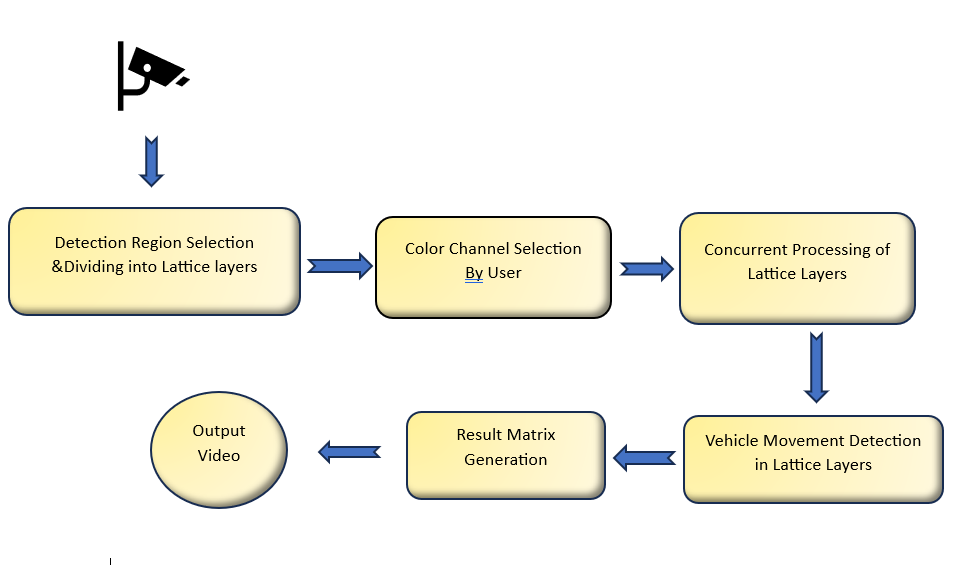
\includegraphics[width=0.9\linewidth]{flowchart.png}
    \caption{Flow Chart}
    \label{fig:enter-label}
\end{figure}


\subsection{The Dataset}\label{AA}
UA-DETRAC is a challenging real-world multi-object detection and multi-object tracking benchmark.The DETRAC Datasets contain highway and normal traffic videos for analysis. 
Surveillance cameras in roads is used and installed worldwide but traffic images are rarely released publicly due to copyright, privacy, and security issues.We are using standard DETRAC datasets to vehicle detection,it will test our model in many ways and conditions.


\subsection{Region Selection}\label{AA}
For selecting the ROI we use opencv techniques.The process of dividing the Region of Interest into smaller grids is an essential part in our method.This method allows for more precise analysis of of vehicles and improves the overall accuracy of detection algorithms.Depending on the type of video and specifications user can select the grid size.

The first step in the process is to identify the Region of Interest (ROI) within the video frame.
We define the Roi by giving the dimensions of x co-ordinate , y-cordinate, grid height
and width. Once the ROI is defined, it is divided into smaller, equally sized grids. The size
of the grid (e.g., 8x8 or 16x16) is chosen based on factors such as the resolution of the video,
the expected size of the vehicles, and computational constraints.
Assume the ROI has a width \( W \) and height \( H \). If the chosen grid size is \( n \times n \), the number of grids along the width and height can be calculated as:
\[
\text{grid\_width} = \frac{\text{roi\_width}}{\text{num\_cols}} = \frac{W}{n}
\]
\[
\text{grid\_height} = \frac{\text{roi\_height}}{\text{num\_rows}} = \frac{H}{n}
\]

Using the dimensions, The coordinates for a grid located at position can be determined as:
\[
\text{start\_grid\_row} = \max\left(0, \frac{(y - \text{roi\_y})}{\text{grid\_height}}\right)
\]
\[
\text{end\_grid\_row} = \min\left(\text{num\_rows} - 1, \frac{(y + h - \text{roi\_y})}{\text{grid\_height}}\right)
\]
\[
\text{start\_grid\_col} = \max\left(0, \frac{(x - \text{roi\_x})}{\text{grid\_width}}\right)
\]
\[
\text{end\_grid\_col} = \min\left(\text{num\_cols} - 1, \frac{(x + w - \text{roi\_x})}{\text{grid\_width}}\right)
\]

After dividing the ROI into grids, the vehicle detection algorithm is applied to each grid independently.The below figure shows the how the lattice layers looks:
\begin{figure}[h]
    \centering
    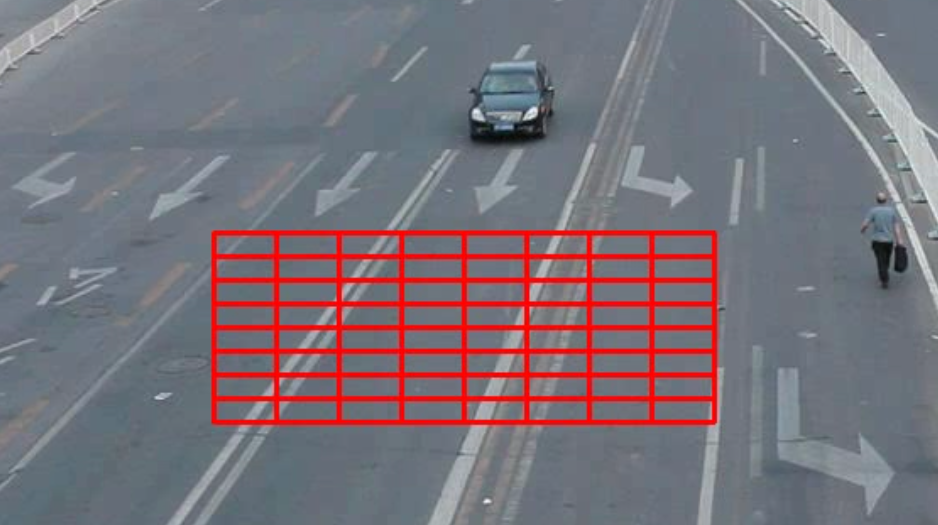
\includegraphics[width=0.7\linewidth]{grid1.png}
    \caption{Lattice View}
    \label{fig:enter-label}
\end{figure}


\subsection{Color Channel processing}
Color channel processing plays an important role in our vehicle detection system by enhancing the detection capabilities through different representations like in color channels.This method uses two primary methods for processing the color information in video frames which is grayscale and HSV channels. Grayscale processing simplifies the computational complexity by reducing the image to a single channel, making it easier to detect motion of the vehicle. On the other hand, HSV processing allows us to use the color information more effectively. By splitting the video frame into its HSV components, we can independently process the hue, saturation, and value channels. This separation helps in detecting vehicles more under varying lighting conditions, as different channels can highlight different aspects of the moving vehicles.if the userschoice is grayscale color channel processing then model converts the image to grayscale and detect the movement or if it is h (or) s (or) v etc.. the detection in lattice is done by and operation of the channels based on user choice user choice can be
\begin{verbatim}
choices = {
    'H': [0],
    'S': [1],
    'V': [2],
    'H+S': [0, 1],
    'H+V': [0, 2],
    'S+V': [1, 2],
    'H+S+V': [0, 1, 2],
    'gray': 'gray'
}
\end{verbatim}

\begin{figure}[h]
    \centering
    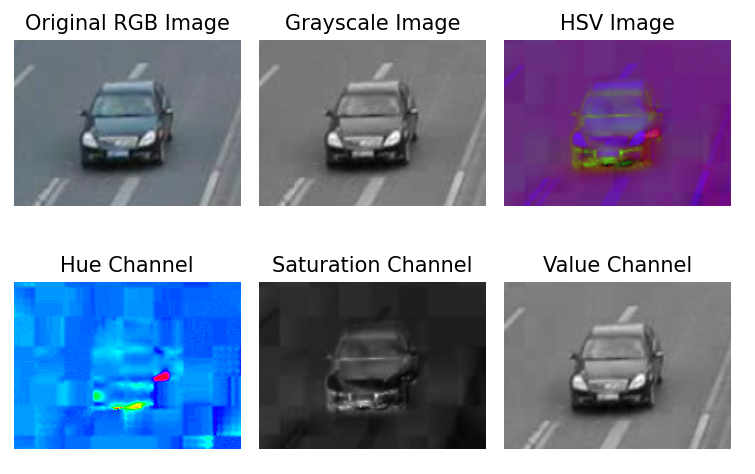
\includegraphics[width=0.8\linewidth]{color channels.png}
    \caption{Color Channels}
    \label{fig:enter-label}
\end{figure}

\subsection{Detection in Grids}
After the Region of Interest is selected, it is divided into an n*n lattice structure, creating smaller regions known as lattice layers. This lattice layer approach allows for more precise analysis of vehicles within the Detection Region. Each lattice layer is analyzed independently to detect the vehicles. The detection process involves many image processing techniques applied to each grid cell, including color channel processing, Gaussian blurring, thresholding, and contour detection. By dividing the Detection region into smaller lattice, the system can process these regions concurrently, enabling parallel processing and improving the overall efficiency and speed of the detection algorithm.

The techniques involved:
\subsubsection{Blurring Image}
To reduce the noise of the image and smoothening the image blur is applied by doing this,the channel is more effective for thresholding and contour detection.

\subsubsection{Thresholding of image}
Thresholding converts the channel into binary,the pixel values are either black or white (0,255)

\subsubsection{Dilation of Image}
this operatiopn helps in expanding the white regions (foreground) in the binary image.This helps in closing the gaps between the contours.

\subsubsection{Contours detection}
This will find the object in the grid and gives the boundaries of the detected part in the grid

\subsection{Processing the grids}
Now we having the coordinates of the grids we should process them individually.There are two ways to process the grids one is sequncially and other is concurrent processing.
\subsubsection{Sequencial processing}
we have the coordinates of lattice,and these lattice are processed to detect a vehicle or part of vehicle in that layer by executing one by one to store the result in a result matrix. The execution takes place on lattice after completing the detection on before lattice.
\subsubsection{concurrent processing}
sequential execution of these grids takes more time,which increases the execution time complexity,so our method uses ThreadPools to execute these lattice.All the grids are passed to ThreadPoolExecutor the coordinates and channels of the grid cell is passed to processing function and it will give result of that gridcell as 1 or 0.

\subsection{Result Matrix Generation}
In our vehicle detection project, we further processed the results from lattice layer object detection to create a binary matrix representing the presence of detected objects within each
lattice.This matrix is updated for each video frame, providing a real-time representation of vehicle locations within the ROI.
The binary matrix, $M$, is created with dimensions $\text{num\_grids\_height} \times \text{num\_grids\_width}$.

Each element M[i][j] in the matrix corresponds to a grid and is set to 1 if an object is detected
in that grid, and 0 otherwise.

\[
\begin{array}{cccccccc}
0 & 0 & 0 & 0 & 0 & 0 & 0 & 0 \\
0 & 0 & 0 & 1 & 1 & 0 & 0 & 0 \\
0 & 0 & 1 & 1 & 1 & 0 & 0 & 0 \\
0 & 0 & 0 & 1 & 1 & 1 & 0 & 0 \\
0 & 0 & 0 & 0 & 0 & 0 & 0 & 0 \\
0 & 0 & 0 & 0 & 0 & 0 & 0 & 0 \\
0 & 0 & 0 & 0 & 0 & 0 & 0 & 0 \\
0 & 0 & 0 & 0 & 0 & 0 & 0 & 0 \\
\end{array}
\]
in this 2D array the results are stored in middle where there is aggregate of ones gives the vehicle.This matrix can also be used to calculate the accuracy results and used to futhur advancements to the project

\section{Results}
After that result matrix is used to show the output results using opencv to draw the rectangles.
The figure below shows the vehicle detection in grids which is represented in green and non detected grids represented in red.

\begin{figure}[h]
    \centering
    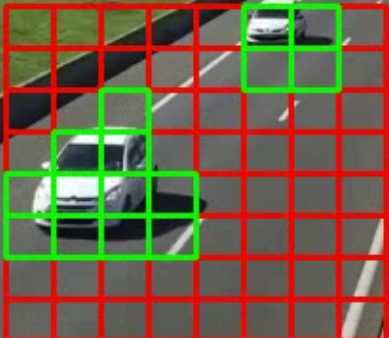
\includegraphics[width=0.6\linewidth]{result1.png}
    \caption{Vehicle Detection}
    \label{fig:vehicle-detection}
\end{figure}

For nearly a 30sec video which the frame count is 680 frames for this when the lattices are executed sequencially the Execution Time is ~52.88 seconds and the Memory Usage is ~106.51 MB for concurrent execution of the grids it is taking Execution Time of ~36.99 seconds Memory Usage of ~112.57 MB



\section{Comparative Results and Analysis}
\subsection{Detection using Concurrent Lattice layers}
We calculated the accuracy of the vehicles frame by frame if the movement in the lattice is detected or not.The lattices are executed concurrently and detect the movement of vehicle.For 200 frames we calculated the accuracy of detections in the lattice.The execution time in (sec) and space Taken in (MB) is also mentioned.

\begin{table}[h]
    \centering
    \begin{tabular}{|c|c|c|c|c|}
        \hline
             & Accuracy & Precision & Execution Time & Space taken(MB) \\
        \hline
        MVI-40712 & 92.89 & 98.2 & 125.98 & 114.15 \\
        \hline
        MVI-39371 & 96.5 & 90.6 & 104.02 & 113.83 \\
        \hline
        MVI-40902 & 88 & 76 & 36.09 & 125.22 \\
        \hline
        MVI-39031 & 65 & 48 & 53.71 & 126.27 \\
        \hline
    \end{tabular}
    \\[1em]
    \caption{Table with Four Rows and Five Columns}
    \label{tab:four-rows-five-columns}
\end{table}

\section{Conclusion}
In this paper we have presented a method for detection of vehicles using concurrent processing of lattice layers in traffic video.
For the application after specifying the Detection Region Co-ordinates and number lattices in the Region the system will detect the movement of vehicle in those lattices.This method ensures the less computation complexity and less time complexity,and has accuracy of around 93.This can be furthur used to estimate the parameters of vehicles and classify the vehicles.

\begin{thebibliography}{00}
\bibitem{b1} JISU KIM. SUNGJUN HONG, and EUNTAI KIM, ``Novel On-Road Vehicle Detection System Using Multi-Stage Convolutional Neural Network,''  June 30, 2021
\bibitem{b2} Ahmad Arinaldi, Jaka Pradana, and Arlan Arventa Gurusinga, ``Detection and classification of vehicles for traffic video analytics,'' Digital Services Division, PT Telekomunikasi Indonesia, Jakarta Pusat 10110, Indonesia.
\bibitem{b3} Mallikarjun Anandhalli, Vishwanath Baligar,Pavana Baligar, Vol. 10, No. 1, March 2021, pp. 66~73.
\bibitem{b4} Haiying Zhang1, Kun Wu1, ``A Vehicle Detection Algorithm Based on Three-Frame Differencing and Background Subtraction,'' Oct 1, 2023 

\bibitem{b5} Nils Defauw,Marielle Malfante, Olivier Antoni, and Tiana Rakotovao, ``Vehicle Detection on Occupancy Grid Maps: Comparison of Five Detectors Regarding Real-Time Performance,'' 2 Febraury 2023
\bibitem{b6} R.Anandhi,G. Sekar, C. Kalaivani, and N. Jayalakshmi, ``Vehicle Detection And System Tracking Using Yolo V3
Model, A Computer Vision Technique,'' November 2, 2022
\bibitem{b7} Agustritus Pasrah Hati Telaumbanua1,Tri Putra Larosa, Panji Dika Pratama, Ra'uf Harris Fauza and Amir Mahmud Husein, ``Vehicle Detection and Identification Using Computer Vision Technology with the Utilization of the YOLOv8 Deep Learning Method,'' Oct 1, 2023
\bibitem{b8} Abderrahim EL BOUZIADY,Rachid OULAD HAJ THAMI, Mounir GHOGHO, Omar BOURJA and Sanaa EL FKIHI, ``Vehicle Speed Estimation usingextracted SURF features from StereoImages,'' 2018 IEEE
\bibitem{b9} Puguh Budi Prakoso,Yuslena Sar, ``Vehicle detection using background subtraction and clustering algorithms,''  June 2019, pp.1393~1398
\bibitem{b10} R. Rajakumar, M. Charan, R. Pandian, T. Prem Jacob, A. Pravin and P. Indumathi , ``Lane Vehicle Detection and Tracking Algorithm Based on Sliding Window,''  28 February 2022 pp 905–919
\bibitem{b11} Genyuan Cheng¹, Yubin Guo², Xiaochun Cheng³, Dongliang Wang, Jiandong Zhao2, ``Real-time Detection of Vehicle Speed Based on Video Image,'' 2020
\bibitem{b12} Cheng-Jian Lin ,2 Shiou-Yun Jeng,3 and Hong-Wei Lioa1, ``A Real-Time Vehicle Counting, Speed Estimation, and Classification System Based on Virtual Detection Zone and Y,'' 2021 pp 10
\bibitem{b13} Khushi Gupta1, Trishul Shrivas2, Siddharth Sharma3, Uma Raj, ``Traffic Management system using Deep Learning ,'' 2023
\bibitem{b14}Shuang Li¹, Faliang Chang¹, Chunsheng Liu1, Nanjun Li¹
, ``Vehicle counting and traffic flow parameter estimation for dense traffic scenes,'' 2023
\bibitem{b15}KEATTISAK SANGSUWAN AND MONGKOL EKPANYAPONG, ``Video-Based Vehicle Speed Estimation Using Speed Measurement Metrics,'' 2024

\end{thebibliography}


\end{document}